\section{引言}
\label{sec:introduction}

长上下文解码需要反复读取完整的键值（KV）历史。对每个生成 token，每个
Query head 都要为全部历史 Key 打分并聚合对应 Value，因此注意力的数据搬运量
和算术量随上下文长度线性增长
\citep{dao2022flashattention,dao2023flashattention2}。KV 淘汰通过永久删除
token 来降低成本
\citep{zhang2023h2o,li2024snapkv,cai2024pyramidkv,feng2024adakv}，但当前
不重要的 token 可能对后续 Query 变得关键。Query-aware 检索则让全部历史保持
可寻址，并在每个 decode step 重新选择一个子集
\citep{tang2024quest,ribar2023sparq,singhania2024loki}。它面临一个严格的
系统约束：寻找子集的成本必须远低于被省去的精确注意力成本。

Token 级低比特检索是一条直接路线。辅助 Key 索引近似所有 QK 分数，top-$k$
确定候选位置，随后精确注意力读取这些位置上的原始 K/V。FIER 表明，即使
1-bit Key 也能保留有用的 token 排序 \citep{wang2025fier}。但是统一 Key
量化器把所有坐标和 attention head 同等对待，而真正影响检索的误差并不是
$\|k-\widehat k\|_2^2$，而是
$(q^\top k-q^\top\widehat k)^2$。只有 Query 各向同性时，这两个目标才等价。
由此产生一个同时具有数值与系统意义的问题：
\emph{在固定索引字节预算下，应如何依据 Query 与 Key 的联合几何分配表示
容量？}

本文提出 \method，一种无需训练、完整精确 KV 驻留 GPU 的检索加速器，来回答
这个问题。对每一层和每个 KV head，参考配置从均匀采样的 prompt Key 与
prompt 尾部 Query 估计 request-local 二阶矩，并分别为 Query 和 Key 构造两个
不同的线性变换。在完整维度下，这两个变换双正交，能够精确保留每一个点积。
在用于构造变换的二阶矩下，两个变换后的二阶矩是相同的对角矩阵。因此，排序
后的坐标刻画的是 QK 联合分数谱，而不是仅由 Key 重建得到的谱。冻结主路径从
当前 prompt 构造这些二阶矩，并在该请求内冻结逐层、逐 head 变换。在互不重叠
校准请求上平均二阶矩得到模型级模板只作为消融评测。

\method 随后把 128 个坐标划分为八个 16 维 band。对每一层和每个 KV head，
它在固定的 240 bit/token/head 预算下，独立为各 band 分配
$0/1/2/4/8$ bit。冻结分配目标是经验 Query 加权 Key 量化误差，它恰好是
attention-logit MSE 的 Cartesian 样本估计。相同 QK-balanced 坐标中的 Key
重建 MSE 简化目标只作为 allocation 消融。0-bit band 在物理上不存储。最终
packed index 每个 token、每个 KV head 占 30 byte，即对应 FP16 K+V 大小的
5.86\%。这是一个\emph{额外的检索索引}：\method 保留全部精确 KV 驻留 GPU，
并不声称物理 KV footprint 只有 1\%。

在每个 decode step，变换后的 INT8 Query 扫描 packed index，并为每个 Query
head 选择
\begin{equation}
 B(N)=\min\{N,1280,\max(256,\lceil0.06N\rceil)\}
 \label{eq:budget-intro}
\end{equation}
个位置。这是已注册的 4K--128K 调度规则，并不表示 1,280-token 上限可以不加
验证地外推到更长上下文。参考配置对所有 proxy score 执行确定性
top-$B(N)$。部署配置使用\cref{eq:frozen-quantile-samples}中的带上限尾部分辨率校准
样本数估计对应阈值，并在扫描过程中直接写出候选，从而避免构造长度为 $N$ 的
score tensor 和调用通用 top-$k$。选中的原始 FP16 K/V 在 GPU 上 gather，并
进入精确稀疏 QK--softmax--AV。系统不使用扩大候选池后的精确 QK 重排、学习式
router、任务族规则、sink/recent 保护启发式或 Full-attention 回退。每项质量
和延迟结果都明确标注其执行配置；我们不会把不同配置的数字拼成同路径结论。
\Cref{fig:overview}给出了完整流程。

在原生极长上下文中，准确选出高分 Key 仍可能不够：大量单独权重很小的遗漏
token 可能携带方向一致的聚合 Value。为此我们注册两个 consumer。
\emph{QKSieve-Fast} 只执行选中集合上的精确注意力；
\emph{QKSieve-Robust} 在同一次索引扫描中额外估计遗漏 proxy 分区和 rank-16
INT4 Value 残差，并以固定 $\alpha=.5$ 与精确选中分子组合。它不增加精确注意力
token，也不使用 router、重排或 Full 回退。Robust 的逐 token 辅助 footprint
为 FP16 K+V 的 7.47\%，Fast 为 5.86\%。

\begin{figure}[t]
  \centering
  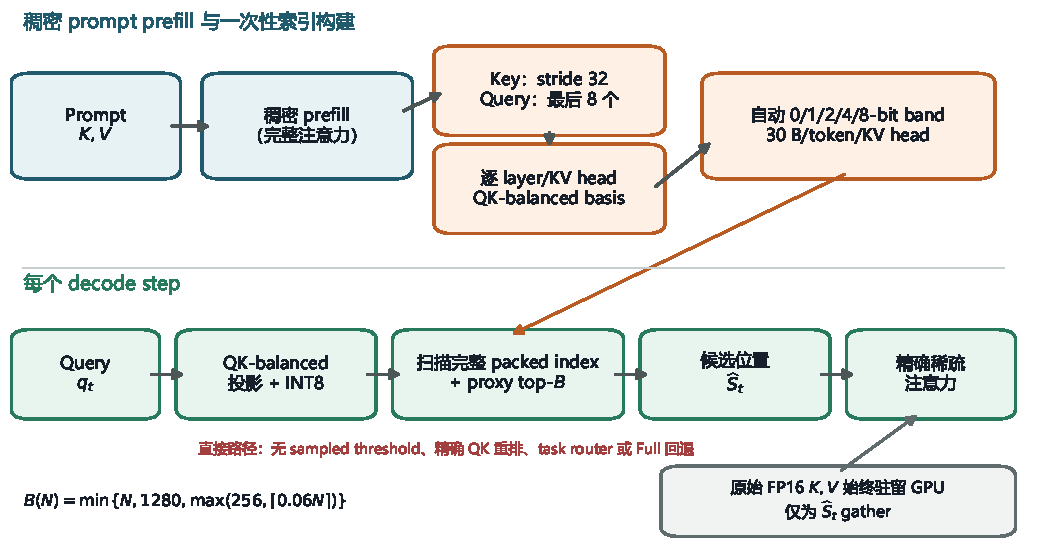
\includegraphics[width=\linewidth]{figures/qksieve_overview_zh.pdf}
  \caption{\method 保留 GPU 上的精确 KV，并增加逐层、逐 KV-head 的混合位宽
  Key 索引。参考配置在 prefill 后冻结 request-local QK-balanced 变换和分配；
  优化配置复用同一 request-local 变换，并使用带上限的 sampled-quantile 候选写出。二者最终都在
  原始 KV 上执行精确稀疏注意力。}
  \label{fig:overview}
\end{figure}

该构造形成了一条清晰的误差链。未量化的坐标变换贡献严格为零的 score 误差。
对 Key 量化误差 $e$，经验 score MSE 是 $\tr(C'_qC_e)$，而不是
$\tr(C_e)$。混合位宽分配器最小化这一量的分 band 版本。score 误差半径与
精确 top-$k$ margin 可以认证必然被保留的 token 子集。最后，若所选集合遗漏
了 Full attention 概率质量 $\epsilon$，则在集合内限制并重新归一化精确
attention 后，概率向量的 $\ell_1$ 变化严格等于 $2\epsilon$，attention 输出
变化至多为 $\epsilon$ 乘以 Value 集合的直径。这些都是条件性保证，而不是
“近似并列的对抗分数一定能保留”的无条件声明。

本文贡献如下：
\begin{itemize}
  \item 推导 QK-balanced 双正交坐标：它精确保留完整点积，并将 Query 与 Key
  二阶矩变换到相同的对角谱。
  \item 将逐层、逐 KV-head 混合位宽索引写成 Query 加权率失真问题，并在
  硬件可见字节预算下，对 16-D band 的 $0/1/2/4/8$ bit 分配求得精确解；
  因果消融比较冻结的 Query-weighted 目标与 Key-MSE。
  \item 实现确定性 packed-index 参考路径和针对 GQA/MHA 架构优化的
  sampled-quantile 部署路径。二者都随后执行 GPU-resident 精确稀疏注意力，
  且均不使用重排、学习式路由或稠密回退。
  \item 识别出独立于 Key 排序的遗漏 Value mass 失真，并提出当前 Query 加权的
  低秩 Value-tail 残差及可解析的收缩偏差--方差关系。Robust 配置在 12 个
  原生 128K 主题/seed case 上保持 99.805\% pooled PPL，case-bootstrap 区间为
  [99.100\%,100.499\%]。Robust 是冻结的长度无关主 consumer；Fast 仅作为
  selected-only 消融。
  \item 给出等索引率检索审计、全层 allocation 统计、GPU kernel 验证和完整
  3,750 样本、16 任务 Llama-3.1-8B LongBench 评测，宏平均分数保持率为
  99.88\%，并给出原生 128K Fast/Robust 压力测试、早期门控消融以及
  8K--128K 的直接 CUDA 和整模型诊断。冻结的原生 MHA 协议下，Fast 与
  Robust 完整 attention 路径分别达到 1.27--6.37$\times$ 与
  1.08--4.12$\times$；Robust 在 32K--128K 的稳态整模型 decode 达到
  1.32--3.98$\times$。通过逐配置报告，将机制、下游质量、attention 子系统
  速度、冷构建和稳态复用严格分开。
\end{itemize}
